
%%%%%%%%%%%%%%%%% Intro %%%
\section{Introduction}
In this report various methods for the estimation of parameters of a given data set are evaluated and compared. To cut down the problem's complexity, we use a simple model for the flux of an elliptic galaxy, as is described by the Sersic profile, which provides us an initial data set. This data set - a noisy image of a elliptic galaxy as it would have been taken by a ground-based telescope - is then used to evaluate different estimation approaches as the least square estimation, maximum likelihood estimation and Bayesian estimation.\\
%Specifically, with these estimators the parameters for the flux of a galaxy is

\section{Modelling a galaxy}
The Sersic profile is very common amongst astrophysicists to model the flux of observed elliptic galaxies in a simple way, and is given by the equation

\begin{equation}
	\centering
	I(l,c) = exp(-R(l,c)^{\frac{1}{n}})
\end{equation}

which describes the variation of intensity with respect to the distance of the galaxy's centre.
The distance $R$ of a pixel with the coordinates $(l,c)$ from the galaxies centre is given by 

\begin{equation}
	\centering
	R(l,c)^2 = \bigg(\frac{(l-l_0)\sin(\alpha) - (c - c_0)\cos(\alpha)}{\sigma_l}\bigg)^2 + \bigg(\frac{(l-l_0)\cos(\alpha) - (c - c_0)\sin(\alpha)}{\sigma_c}\bigg)^2
\end{equation}

with $(l_0,c_0)$ being the galaxy's centre coordinates, $(\sigma_l,\sigma_c)$ the two galaxy's axes length and the horizontal angle $\alpha$.

This leads to the following equation modelling the data

\begin{equation}
	\centering
	d(l,c) = s + a I(l,c) + n(l,c)
\label{eq:dlc}
\end{equation}

with $a$ as the amplitude of the galaxy, $s$ the amplitude of the sky's background and $n(l,c)$ as noise.


Using the Sersic profile we can now generate an artificial elliptic galaxy, see \cref{fig:initial}.


\begin{figure}[!h]
	\centering
	\begin{minipage}[b]{0.4\textwidth}
		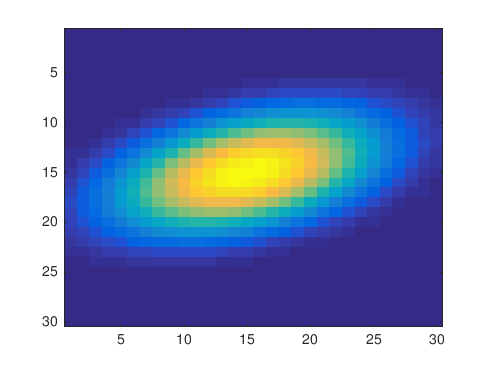
\includegraphics[width=\textwidth]{images/galaxy_initial}
		\caption{Initial data set}
		\label{fig:initial}
	\end{minipage}
	\begin{minipage}[b]{0.4\textwidth}
		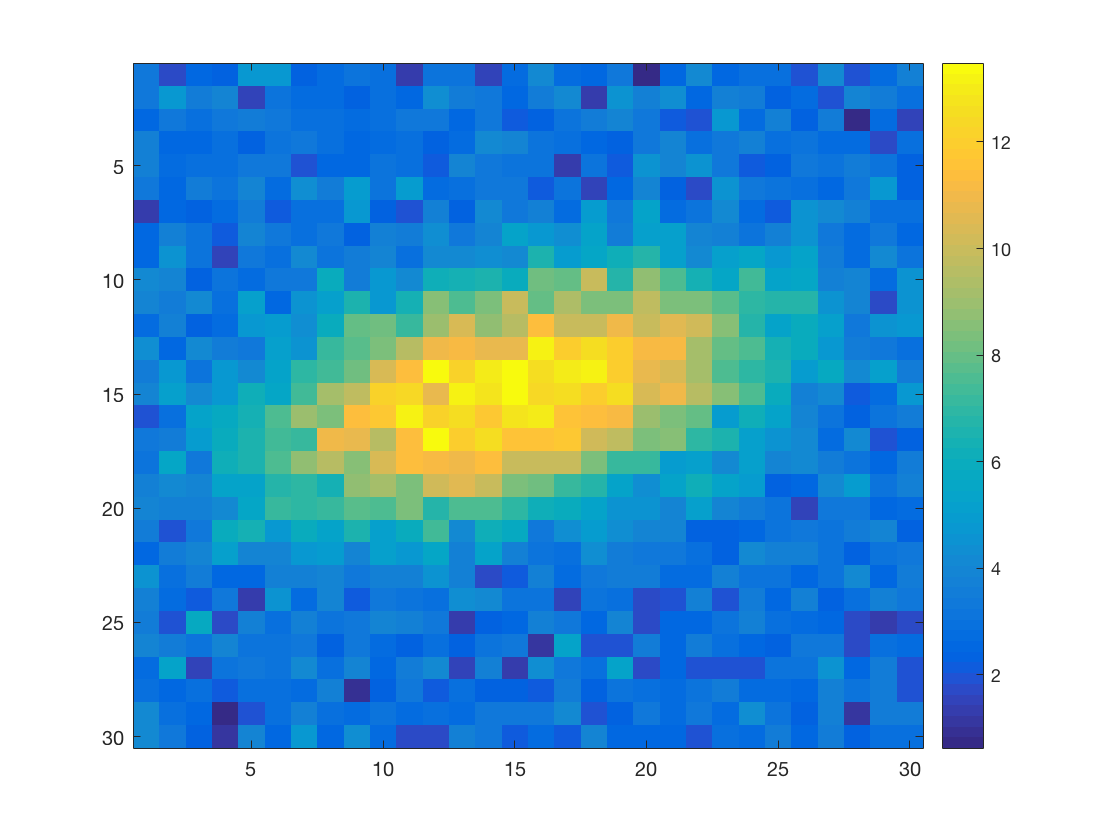
\includegraphics[width=\textwidth]{images/galaxy_noise}
		\caption{Random noise added}
		\label{fig:addedNoise}
	\end{minipage}
\end{figure}

By assuming a Gaussian white noise with the known variance $\sigma_n^2$ and using the initial image of the galaxy, we can model the elliptic galaxy as it would have been seen by a ground-based telescope, see \cref{fig:addedNoise}.



The parameters used to create above mentioned figure are given as follows


	\begin{align*}
		L, C & = 30 & l_0, c_0 & = 15 & \sigma_l & = 10 & \sigma_c & = 5 & \sigma_n & = 0.8 \\
		\alpha & = 0.3 & n & = 0.5 & a & = 10 & s & = 3 
	\end{align*}

with $L,C$ as height respectively width of image in pixels and $\sigma_n$ as the standard deviation of the gaussian white noise.




%%%%%%%%%%%%%%%%% TASK 1 %%%
\section{Estimation with known Galaxy's location and shape parameters}
Having successfully modelled a simple elliptic galaxy, this model is used as input data for the simulation of an estimation of the galaxy's and sky background's amplitude, while assuming that the galaxy's position and shape parameters are known. This estimation can be formulated via:
\begin{equation}
\boldsymbol{y}=\boldsymbol{H}\boldsymbol{\theta}+\boldsymbol{n}(c,l)
\label{eq:generalestimation}
\end{equation}
Here, $\boldsymbol{y}$ is the actual measurement, in our case it is the intensity of the galaxy. However, one has to keep in mind that for the  following steps, we use the simulated galaxy intensity as described above as our measured galaxy intensity. $\boldsymbol{\theta}$ is the vector of estimated parameters, which are in our case the galaxy's amplitude $a$ and the background's amplitude $s$, so $\boldsymbol{\theta}=[s,a]^{\mathrm{T}}$. $\boldsymbol{H}$ is a matrix describing the underlying model, which in our case also depends on the pixel position since the intensity described by the sersic function depends on the distance towards the centre of the galaxy, and $\boldsymbol{n}(l,c)$ is a noise component also depending on the pixel position (l,c). In order to satisfy equation \ref{eq:dlc} using equation \ref{eq:generalestimation}, one has to define $\boldsymbol{H}$ in a special matrix form, which is given by:
\begin{equation}
H_{l,c}=\left(\begin{array}{cc}1& \exp(-R_{l,c}^{\frac{1}{n}}) \end{array}\right)\\
\end{equation}
Thus, $\boldsymbol{H}$ is a $2\times (L\cdot C)$ matrix, describing the intensity profile of the galaxy for each pixel (l,c). Therefore, our data $\boldsymbol{d}$ describing the measured data for all pixels yields:
\begin{equation}
\boldsymbol{d}=\boldsymbol{H}\boldsymbol{\theta}+\boldsymbol{n}(c,l),
\label{eq:generalestimation}
\end{equation}
where $d$ is a vector with $L\cdot C$ elements.\\
\newline
In order the obtain maximum likelihood estimator for $\boldsymbol{\theta}$ as a function of $\boldsymbol{d}$, one has to calculate:
\begin{equation}
\boldsymbol{\theta}=\left(\boldsymbol{H'H}\right)^{-1}\cdot\boldsymbol{H}\cdot\boldsymbol{d}
\end{equation}
The bias of that estimator could be calculated using $b_{\boldsymbol{\theta}}(\boldsymbol{\theta}_{init})=E_{Y|\boldsymbol{\theta}_{init}}(\boldsymbol{\theta})-\boldsymbol{\theta}_{init}$, where $\boldsymbol{\theta}_{init}$ is the vector of the true parameters that we want to find out. However, this bias is only applicable for a larger sets of simulations.
The used matlab code performing this is shown in the appendix. The resulting maximum likelihood estimators for the galaxy's and the sky background's amplitudes are:
\begin{equation*}
\boldsymbol{\theta}=\left[2.9576\;10.0131 \right]^{\mathrm{T}}
\end{equation*}
This result is very close to the original parameters used for the simulation of the data with $ \boldsymbol{\theta}_{initial}=\left[3\;10 \right]^{\mathrm{T}}$ (see list of parameters above). However, we assumed the galaxy center and shape to be known, which drastically reduces the number of unknowns in this fit, and therefore results in a very good fit result.

%%%%%%%%%%%%%%%%% TASK 2 %%%
\section{Maximum likelihood estimation of all parameters}
In the next step, we assumed that the galaxy's position and shape are unknown for the fit. Thus, now also the parameter vector $\boldsymbol{\nu}=\left[l_{0},c_{0}, \sigma_{l}, \sigma_{c},n\right]$ also needs to be fitted simultaniously to $\theta$. Again, the corresponding model can be formulated as:
\begin{equation*}
\boldsymbol{d}=\boldsymbol{H}(\boldsymbol{\nu})\boldsymbol{\theta}+\boldsymbol{n}(c,l),
\end{equation*}
The only difference now is that $\boldsymbol{H}$ depends on the variable $\boldsymbol{\nu}$. Again, $\boldsymbol{H}$ is a $2\times(\L\cdot C)$ - matrix, $\theta=\left[s,a\right]^{\mathrm{T}}$, $\boldsymbol{d}$ a vector with $L\cdot C$ components and $\$\boldsymbol{\nu}$ as defined above a vector with six components. The goal is to obtain the maximum likelihood estimator by minimizing the quadratic cost function $\boldsymbol{J}$:

\begin{equation}
\boldsymbol{J}(\boldsymbol{\theta,\nu})=\left(\boldsymbol{d}-\boldsymbol{H}(\boldsymbol{\nu})\boldsymbol{\theta}\right)^{\mathrm{T}}\left(\boldsymbol{d}-\boldsymbol{H}(\boldsymbol{\nu})\boldsymbol{\theta}\right)
\label{eq:costfunction}
\end{equation}
The optimization problem thus is a least square optimization. The maximum likelihood estimators are then given by:
\begin{equation*}
\left(\boldsymbol{\theta}_{ML},\boldsymbol{\nu}_{ML}\right)=argmin\left(\boldsymbol{J}\right)
\end{equation*}

For a large number of samples, this maximum likelihood estimator is unbiased with a variance equal to the inverse of the Fisher matrix: $\boldsymbol{\sigma}^{2}=\boldsymbol{F}(\boldsymbol{\theta})^{-1}$

%%%%%% arty part form here

The simplest method to gain initial parameters for the optimisation is to perform an "educated guess" \todo{phrasing} using the obtained noisy image from the galaxy. More specifically, the galaxy's centre and the amplitude of the galaxy as well as the background noise can be read straight from the image within a reasonable error-range. However, the shape and form of the galaxy can not be read out or estimated directly since the present noise can not be estimated with a reasonable accuracy. Thus we use arbitrary values for the shape parameters.\\
These initial parameters can then be used to compute a cost function, c.f. \cref{Appendix C}, which then can be minimised to obtain an optimal set of parameters based on the initial ones. Re-inserting the former into the Sersic model, we can generate an estimation of the true galaxy (c.f. \cref{fig:initial}), as can be seen in \cref{fig:MLE}.


\begin{table}[h!]
\centering
\begin{tabular}{ l | c c c c c c c c}
	& $s$ & $a$ & $l_0$ & $c_0$ & $\sigma_l$ & $\sigma_c$ & $\alpha$ & $n$ \\
	\hline
	initial & 1 & 20 & 14 & 17 & 1 & 1 & 1 & 1 \\
	estimated & 3.0660 & 9.8379 & 14.9496 & 15.0309 & 10.0970 & 5.0054 & 0.2978 & 0.4922 \\
	theoretical & 3 & 10 & 15 & 15 & 10 & 5 & 0.3 & 0.5
\end{tabular}
\caption{parameter comparison}
\label{tab:param}
\end{table}

\begin{figure}[h!]
	\centering
	\begin{minipage}[b]{0.4\textwidth}
		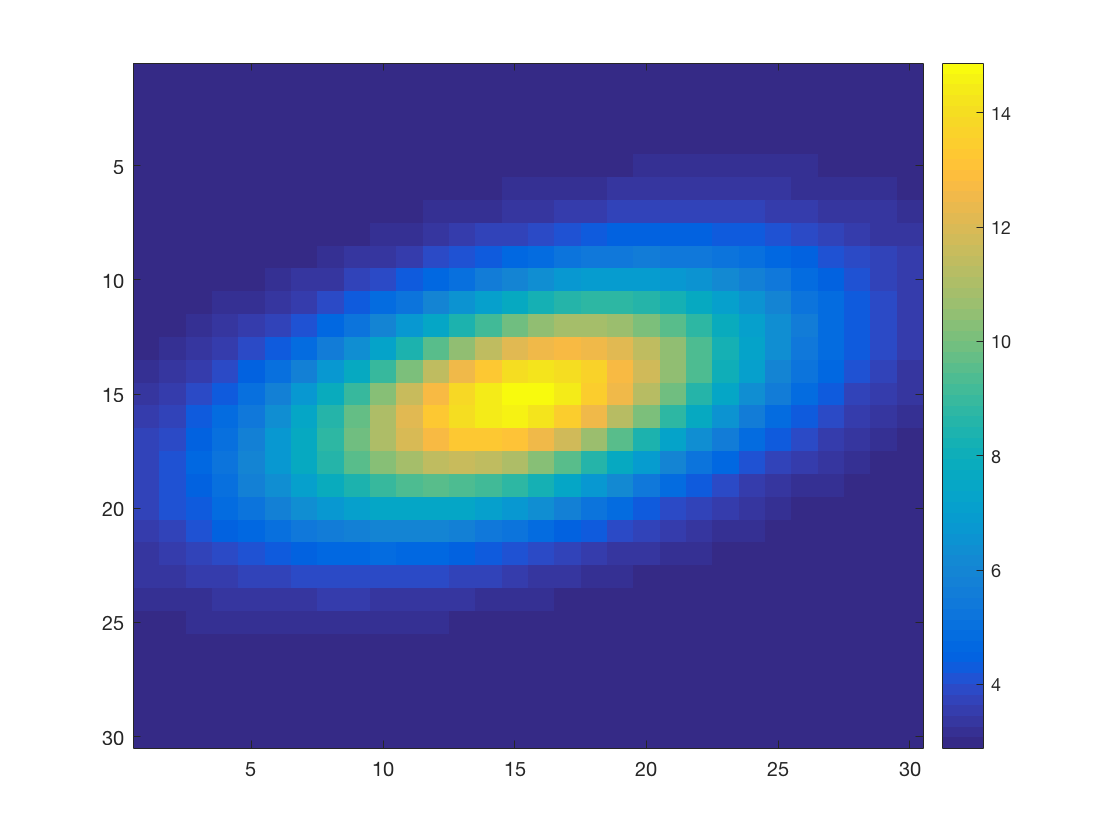
\includegraphics[width=\textwidth]{images/galaxy_MLE}
		\caption{estimated galaxy}
		\label{fig:MLE}
	\end{minipage}
	\begin{minipage}[b]{0.4\textwidth}
		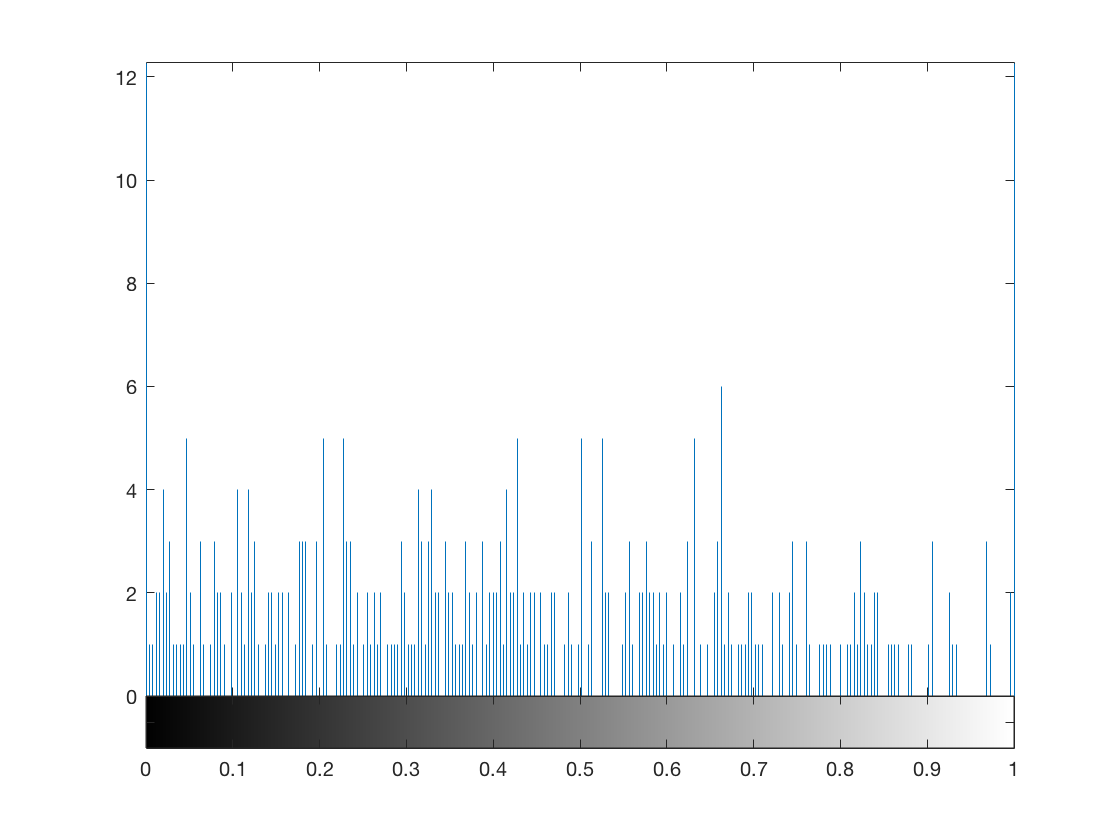
\includegraphics[width=\textwidth]{images/residual_histogram}
		\caption{Histogram of residual data}
		\label{fig:residual}
	\end{minipage}
\end{figure}

As can be seen in \cref{tab:param}, the estimated parameters are extremely close to the theoretical ones that were used to obtain \cref{fig:initial}, our initial image of the elliptic galaxy. This results in an image (c.f. \cref{fig:MLE}) of the galaxy that is very similar to the initial one, even though the initially guessed parameters were not chosen close to the theoretical ones.

Since this optimisation approach is very susceptible to the initial parameter guess, it is not guaranteed that this approach will succeed and result in physically reasonable optimal parameters. To avoid this behaviour in practice, the initial parameters can be altered until they are within an acceptable range or the optimisation process can be modified such that physically unreasonable parameters are rejected during the process - which adversely would increase the complexity of the whole process.

By subtracting the image created with the estimated parameters from the noisy image presumably obtained by the telescope (\cref{fig:addedNoise}), we obtain the so-called "residuals", which correspond to the noise that is included in the obtained image.
Considering the histogram of these residuals as shown in \cref{fig:residual} and by calculating the standard deviation (c.f. Matlab code in \cref{Appendix B}), the noise seems to be compatible with our model for the noise - a simple white gaussian noise - since the histogram shows a more or less even distribution of numerical data and the standard deviation of $0.7949$ is very close to our initially introduced value of $\sigma = 0.8$.



However, varying the initial parameters for the optimisation can result in unusable data - which can not even be interpreted as elliptic galaxy anymore, especially if the initial parameters are too different from the theoretical ones. The closer the parameters are chosen to their respective theoretical value the better the maximum likelihood estimation performs.


% residual standard deviation: 0.7949
%parameters for that image:    
%    3.0660
%    9.8379
%   14.9496
%   15.0309
%   10.0970
%    5.0054
%    0.2978
%    0.4922
% guessed parameters:
%     1
%    20
%    14
%    17
%     1
%     1
%     1
%     1
% theoretical parameters:
%l0 = floor(L/2);
%c0 = floor(C/2);
%sigma_l = 10;
%sigma_c = 5;
%alpha = 0.3;
%n = 0.5;
%a = 10;
%s = 3;


%%%%%%%%%%%%%%%%% TASK 3 %%%
\section{Estimation in the Bayesian framework}




\subsection{Maximum a posteriori estimator}

\subsection{Posterior mean estimator}


